% Usage: knitr slide


\chapter{Diagnosis}\blfootnote{Most of this material is from
  ``Direct Measures of Diagnostic Utility Based on Diagnostic Risk Models`` by FE Harrell presented at the FDA Public Workshop on Study Methodology for Diagnostics in the Postmarket Setting, 2011-05-12.}\movie{https://www.youtube.com/watch?v=uULhuuSjBww}

Medical diagnostic research, as usually practiced, is prone to bias
and even more importantly to yielding information that is not useful
to patients or physicians and sometimes overstates the value of
diagnostic tests.  Important sources of these problems are conditioning on
the wrong statistical information, reversing the flow of time, and
categorization of inherently continuous test outputs and disease
severity.  It will be shown that sensitivity and specificity are not
properties of tests in the usual sense of the word, and that
they were never natural choices for describing
test performance.  This implies that ROC curves are unhelpful
(although areas under them are sometimes useful).  So is
categorical thinking.

This chapter outlines the many advantages of diagnostic risk modeling,
showing how pre-- and post-test diagnostic models give
rise to clinically useful displays of pre-test vs.\ post-test
probabilities that themselves quantify diagnostic utility in a way
that is useful to patients, physicians, and diagnostic device makers.
And unlike sensitivity and specificity, post-test probabilities are
immune to certain biases, including workup bias.

Case-control studies use a design where sampling is done on final disease
status and patient exposures are ``along for the ride.''  In other
words, one conditions on the outcome and considers the distribution of
exposures using outcome-dependent sampling.  Sensitivity and
specificity are useful for proof-of-concept case-control studies
because sensitivity and specificity also condition on the final diagnosis.
The use of sensitivity and specificity in prospective cohort studies
is the mathematical equivalent of making three left turns in order to
turn right.   Like the complex adjustments needed for $P$-values when
doing sequential trials, sensitivity and specificity require complex
adjustments for workup bias just because of their backward
consideration of time and information.  In a cohort study one can use
a vanilla regression model to estimate the probability of a final
diagnostic outcome given patient characteristics and diagnostic test results. 


\section{Problems with Traditional Indexes of Diagnostic Utility}

sensitivity = Prob$[T^{+} | D^{+}]$\\
\bigskip
specificity = Prob$[T^{-} | D^{-}]$\\
\bigskip
Prob$[D^{+} | T^{+}] = \frac{sens \times prev}{sens \times prev +
(1-spec)\times (1-prev)}$

Problems:
\bi
\item Diagnosis forced to be binary
\item Test force to be binary
\item Sensitivity and specificity are in backwards time order
\item Confuse decision making for groups vs.\ individuals
\item Inadequate utilization of pre-test information
\item Dichotomization of continuous variables in general
\ei

\subsubsection{Example: BI-RADS Score in Mammography}
Does Category 4 Make \textbf{Any} Sense?

\begin{center}\smaller[2]\begin{tabular}{|l|l|l|} \hline
 & \textbf{Diagnosis} & \textbf{Number of
Criteria\footnote{Breast Imaging Reporting and Data System, American
  College of Radiologists
  \url{http://breastcancer.about.com/od/diagnosis/a/birads.htm}. American
  College of Radiology. BI-RADS US (PDF document) Copyright
  2004. BI-RADS US. arc.org}} \\ \hline
0 & Incomplete & \parbox{2.25in}{Your mammogram or ultrasound didn't give the
radiologist enough information to make a clear diagnosis; follow-up
imaging is necessary} \\ \hline
1 & Negative & \parbox{2.25in}{There is nothing to comment on; routine
screening recommended}\\ \hline
2 & Benign   & \parbox{2.25in}{A definite benign finding; routine screening
recommended}\\ \hline
3 & \parbox{1.25in}{Probably Benign} & \parbox{2.25in}{Findings that have
a high probability of being benign ($>98$\%); six-month short interval
follow-up}\\ \hline
4 & \parbox{1.25in}{Suspicious Abnormality} & \parbox{2.25in}{Not characteristic of breast cancer, but
reasonable probability of being malignant (3 to 94\%); biopsy should
be considered}\\ \hline
5 & \parbox{1.25in}{Highly Suspicious of Malignancy} & \parbox{2.25in}{Lesion that has a high
probability of being malignant ($\geq 95$\%); take appropriate
action}\\ \hline
6 & \parbox{1.25in}{Known Biopsy Proven Malignancy} & \parbox{2.25in}{Lesions known to be malignant
that are being imaged prior to definitive treatment; assure that
treatment is completed}\\ \hline
\end{tabular}\end{center}


How to Reduce False Positives and Negatives?
\bi
\item Do away with ``positive'' and ``negative''
\item Provide risk estimates
\item Defer decision to decision maker
\item Risks have self-contained error rates
\item Risk of 0.2 $\rightarrow$ Prob[error]=.2 if don't treat
\item Risk of 0.8 $\rightarrow$ Prob[error]=.2 if treat
\ei

See
\url{http://thehealthcareblog.com/blog/2015/12/01/rethinking-about-diagnostic-tests-there-is-nothing-positive-or-negative-about-a-test-result}
for a nice article on the subject.

\subsubsection{Binary Diagnosis is Problematic Anyway}
\quoteit{The act of diagnosis requires that patients be placed in a binary
category of either having or not having a certain
disease. Accordingly, the diseases of particular concern for
industrialized countries---such as type 2 diabetes, obesity, or depression---require that
a somewhat arbitrary cut-point be chosen on a continuous scale of
measurement (for example, a fasting glucose level $>6.9$ mmol/L
[$>125$ mg/dL] for type 2 diabetes). These cut-points do not
adequately reflect disease biology, may inappropriately treat patients 
on either side of the cut-point as 2 homogeneous risk groups, fail to
incorporate other risk factors, and are invariable to patient
preference.}{\citet{vic08aga}}

\subsubsection{Back to Sensitivity and Specificity}
\bi
\item Backwards time order
\item Irrelevant to both physician and patient
\item Improper discontinuous scoring rules\footnote{They are optimized
    by not correctly estimating risk of disease.}
\item Are not test characteristics
 \bi
 \item Are characteristics of the test \textbf{and} patients
 \ei
\item \textbf{Not constant}; vary with patient characteristics
 \bi
 \item Sensitivity $\uparrow$ with any covariate related to disease
 severity if diagnosis is dichotomized
 \ei
\item Require adjustment for workup bias
 \bi
 \item Diagnostic risk models do not; only suffer from under-representation
 \ei
\item Good for proof of concept of a diagnostic method in a
 case--control study; not useful for utility
\ei

\citet{hla84fac}; \cite{moo97lim}; \citet{moo03sen}; \citet{gne07str}

\subsubsection{Sensitivity of Exercise ECG for Diagnosing CAD}
\begin{center}\smaller
\begin{tabular}{lr} \hline
\textbf{Age} (years) & \textbf{Sensitivity} \\
~~~~$<40$ & 0.56 \\
~~~~40--49& 0.65 \\
~~~~50--59 & 0.74 \\
~~~~$\geq$ 60 & 0.84 \\ \hline
\textbf{Sex} & \\
~~~~male & 0.72 \\
~~~~female & 0.57 \\ \hline
\textbf{\# Diseased CAs} & \\
~~~~1 & 0.48 \\
~~~~2 & 0.68 \\
~~~~3 & 0.85 \\ \hline
\end{tabular}\end{center}
\citet{hla84fac}

\section{Problems with ROC Curves and Cutoffs}
{\smaller \ldots statistics such as the AUC are not especially relevant to someone who
must make a decision about a particular $x_{c}$.  \ldots ROC curves
lack or obscure several quantities that are necessary for evaluating
the operational effectiveness of diagnostic tests. \ldots ROC curves
were first used to check how radio \emph{receivers} (like radar
receivers) operated over a range of frequencies. \ldots This is not
how most ROC curves are used now, particularly in medicine.  The
receiver of a diagnostic measurement \ldots wants to make a decision
based on some $x_{c}$, and is not especially interested in how well he
would have done had he used some different cutoff.~\citet{bri08ski}
\\[1ex]
\hrule
In the discussion to this paper, David Hand
states ``when integrating to yield the overall 
AUC measure, it is necessary to decide what weight to give each value
in the integration.  The AUC implicitly does this using a weighting
derived empirically from the data.  This is nonsensical.  The relative 
importance of misclassifying a case as a non-case, compared to the
reverse, cannot come from the data itself.  It must come externally,
from considerations of the severity one attaches to the different
kinds of misclassifications.''}

\section{Optimum Individual Decision Making and Forward Risk}
\bi
\item Minimize expected loss/cost/disutility
\item Uses
 \bi
 \item utility function (e.g., inverse of cost of missing a diagnosis, cost of
 over-treatment if disease is absent)
 \item probability of disease
 \ei
\ei
$d =$ decision, $o =$ outcome\\
Utility for outcome $o = U(o)$\\
Expected utility of decision $d = U(d) = \int p(o | d) U(o)do$\\
$d_{\textrm opt} = d$ maximizing $U(d)$

The steps for determining the optimum decision are:
\be
\item Predict the outcome $o$ for every decision $d$
\item Assign a utility $U(o)$ to every outcome $o$
\item Find the decision $d$ that maximizes the expected utility
\ee

See
\bi
\item \url{http://en.wikipedia.org/wiki/Optimal_decision}
\item \url{http://www.statsathome.com/2017/10/12/bayesian-decision-theory-made-ridiculously-simple}
\item \url{https://twitter.com/jim_savage_/status/989524417649807360}
\item Govers~\etal~\cite{gov18int}
\item \url{https://stats.stackexchange.com/questions/368949}
\ei

% From Chris Fonnesbeck 2015-10-26:
% The way decision analysts approach the problem is by considering the expected value of perfect information (EVPI), or in this case, the expected value of sample information (EVSI). It quantifies the value of additional information essentially by differencing the average of optimal values from the optimum of the average expected value. EVPI is related to the value of learning about an underlying model, whereas EVSI is the value of collecting additional data. Estimating the loss of information due to discretization would just be a special case of an EVSI calculation.

See
\href{https://www.nytimes.com/2018/09/01/opinion/sunday/how-make-big-decision.html}{this NY Times article} about decision theory.

\section{Diagnostic Risk Modeling}
Assuming (Atypical) Binary Disease Status
\begin{center}\smaller
\begin{tabular}{ll}
$Y$ & 1:diseased, 0:normal\\
$X$ & vector of subject characteristics {\smaller[3] (e.g., demographics,
risk factors, symptoms)} \\
$T$ & vector of test (biomarker, \ldots) outputs\\
$\alpha$ & intercept\\
$\beta$ & vector of coefficients of $X$\\
$\gamma$ & vector of coefficients of $T$
\end{tabular}
\\[2ex]
\smaller[-1]
pre$(X)$ = Prob$[Y=1 | X] = \frac{1}{1 + \exp[-(\alpha^{*} + \beta^{*} X)]}$ \\
post$(X,T)$ = Prob$[Y=1 | X,T] = \frac{1}{1 + \exp[-(\alpha + \beta X + \gamma T)]}$
\end{center}

Note: Proportional odds model extends to ordinal disease severity $Y$.

\subsection{Example Diagnostic Models}
\begin{figure}[!htbp]\leavevmode
\centerline{\includegraphics[width=.8\textwidth]{cad-nomo.pdf}}
\caption{\large A nomogram for estimating the likelihood of significant
 coronary artery disease (CAD) in women.  ECG = electrocardiographic;
 MI = myocardial infarction.~\protect\cite{pry83}  Reprinted from
 American Journal of Medicine, Vol.\ 75, D.B.\ Pryor~\etal, ``Estimating
 the likelihood of significant coronary artery disease,'' p.\ 778,
 Copyright 1983, with permission from Excerpta Medica, Inc.}
\end{figure}

\begin{figure}[!htbp]\leavevmode%
\centerline{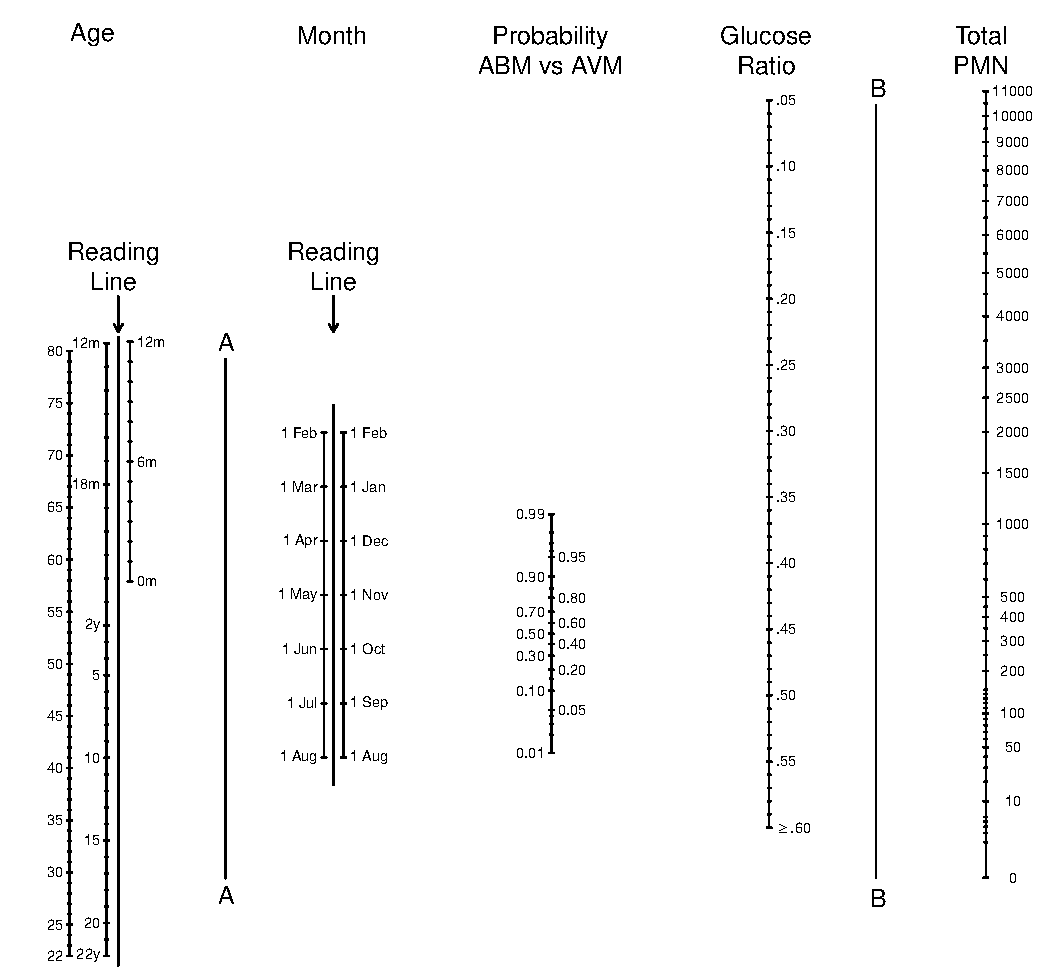
\includegraphics[width=.9\textwidth]{abm-nomo.pdf}}
\caption{Nomogram for estimating probability of bacterial (ABM) versus viral (AVM) meningitis.  Step 1, place ruler on reading lines for patient's 
age and month of presentation and mark intersection with line A; step 2,
place ruler on values for glucose ratio and total polymorphonuclear
leukocyte (PMN) count in cerebrospinal fluid and mark intersection with line
B; step 3, use ruler to join marks on lines A and B, then read off the
probability of ABM versus AVM.  From~\protect\citet{spa89}}
\end{figure}

\begin{figure}[!htbp]\leavevmode%
\centerline{\includegraphics[width=.8\textwidth]{bra91usiNomogram.png}}
\caption{Proportional odds ordinal logistic model for ordinal diagnostic classes from~\citet{bra91usi}}
\end{figure}
\clearpage

\section{Assessing Diagnostic Yield}
\subsection{Absolute Yield}
\citet{pen08eva}: Absolute incremental information in a new set of
markers\\
Consider change in predicted risk when add new variables\\
\bigskip
\hrule
\medskip
Average increase in risk of disease when disease present\\~~~~~~~~~~~~~~~~~~~~~~~~~~~~~~~~~~~~+\\
Average decrease in risk of disease when disease absent\\
\medskip

\subsubsection{Formal Test of Added Absolute and Relative Information}
Likelihood ratio $\chi^{2}$ test of partial association
of new markers, adjusted for old markers

\subsection{Assessing Relative Diagnostic Yield}
\bi
\item Variation in relative log odds of disease = $T \hat{\gamma}$,
holding $X$ constant
\item Summarize with Gini's mean difference or inter-quartile range,
then anti-log
\item E.g.: the typical modification of pre-test odds of disease is by
a factor of 3.4
\ei
{\smaller Gini's mean difference = mean absolute difference between any
pair of values}

See Figure~\ref{fig:ancova-or-diff} for a graphical depiction of the relationship between odds ratio and absolute risk difference.

\section{Assessing Absolute Diagnostic Yield: Cohort Study}
\bi
\item Patient $i = 1, 2, 3, \ldots, n$
\item In-sample sufficient statistics: pre$(X_{1})$, \ldots,
pre$(X_{n})$, post$(X_{1}, T_{1})$, \ldots, post$(X_{n}, T_{n})$
\ei

\begin{figure}[!htbp]\leavevmode
\centerline{\includegraphics[width=.8\textwidth]{hla09criFig3.png}}
\caption{Pre vs.\ post-test probability.  This may be ummarized with quantile regression to estimate 0.1 and 0.9 quantiles of \textbf{post} as a function of \textbf{pre}.  From~\citet{hla09cri}}
\end{figure}

Assessments assume that risk estimates are well calibrated, using, for example a high-resolution continuous calibration curve.

\centerline{\includegraphics[width=.8\textwidth]{ordinal-calibrate-1}}

Out-of-sample assessment: compute pre$(X)$ and post$(X,T)$ for
any $X$ and $T$ of interest
\subsubsection{Summary measures}
 \bi
 \item quantile regression {\smaller[2](\cite{koe78reg})} curves as a function of pre
 \item overall mean $|$post -- pre$|$
 \item quantiles of post -- pre
 \item du$_{50}$: \textbf{distribution} of post when pre = 0.5 \\
 diagnostic utility at maximum pre-test uncertainty 
  \bi
  \item Choose $X$ so that pre = 0.5
  \item Examine distribution of post at this pre
  \item Summarize with quantiles, Gini's mean difference on prob.\
 scale
  \item Special case where test is binary (atypical): compute post for
 $T^{+}$ and for $T^{-}$
  \ei
\ei

\section{Assessing Diagnostic Yield: Case-Control \& Other Oversampling Designs}
\bi
\item Intercept $\alpha$ is meaningless
\item Choose $X$ and solve for $\alpha$ so that pre = 0.5
\item Proceed as above to estimate du$_{50}$
\ei

\section{Example: Diagnosis of Coronary Artery Disease (CAD): Test = Total
Cholesterol}
\begin{Schunk}
\begin{Sinput}
require(rms)
\end{Sinput}
\begin{Sinput}
getHdata(acath)
acath <- subset(acath, !is.na(choleste))
dd <- datadist(acath);  options(datadist='dd')
f <- lrm(sigdz ~ rcs(age,5)*sex, data=acath)
pre <- predict(f, type='fitted')
g <- lrm(sigdz ~ rcs(age,4)*sex + rcs(choleste,4) + rcs(age,4) %ia%
         rcs(choleste,4), data=acath)
ageg <- c(40, 70)
psig <- Predict(g, choleste, age=ageg)
s <- lrm(tvdlm ~ rcs(age,4)*sex + rcs(choleste,4) + rcs(age,4) %ia%
	rcs(choleste,4), data=acath)
psev <- Predict(s, choleste, age=ageg)
ggplot(rbind('Significant CAD'=psig, '3 Vessel or Left Main CAD'=psev),
	adj.subtitle=FALSE)
\end{Sinput}
\begin{figure}[htbp]

\centerline{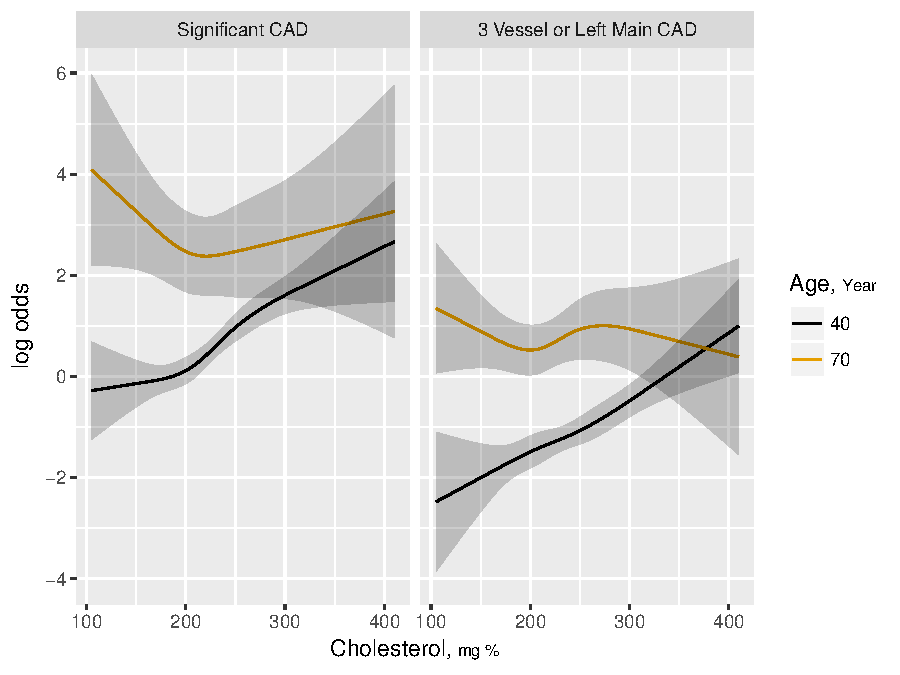
\includegraphics[width=\maxwidth]{dx-du-1} }

\caption[Relative effect of total cholesterol for age 40 and 70]{Relative effect of total cholesterol for age 40 and 70; Data from Duke Cardiovascular Disease Databank, $n=2258$}\label{fig:dx-du}
\end{figure}
\end{Schunk}
\clearpage
\begin{Schunk}
\begin{Sinput}
post <- predict(g, type='fitted')
plot(pre, post, xlab='Pre-Test Probability (age + sex)',
     ylab='Post-Test Probability (age + sex + cholesterol)', pch=46)
abline(a=0, b=1, col=gray(.8))
lo <- Rq(post ~ rcs(pre, 7), tau=0.1)  # 0.1 quantile
hi <- Rq(post ~ rcs(pre, 7), tau=0.9)  # 0.9 quantile
at <- seq(0, 1, length=200)
lines(at, Predict(lo, pre=at)$yhat, col='red', lwd=1.5)
lines(at, Predict(hi, pre=at)$yhat, col='red', lwd=1.5)
abline(v=.5, col='red')
\end{Sinput}
\begin{figure}[htbp]

\centerline{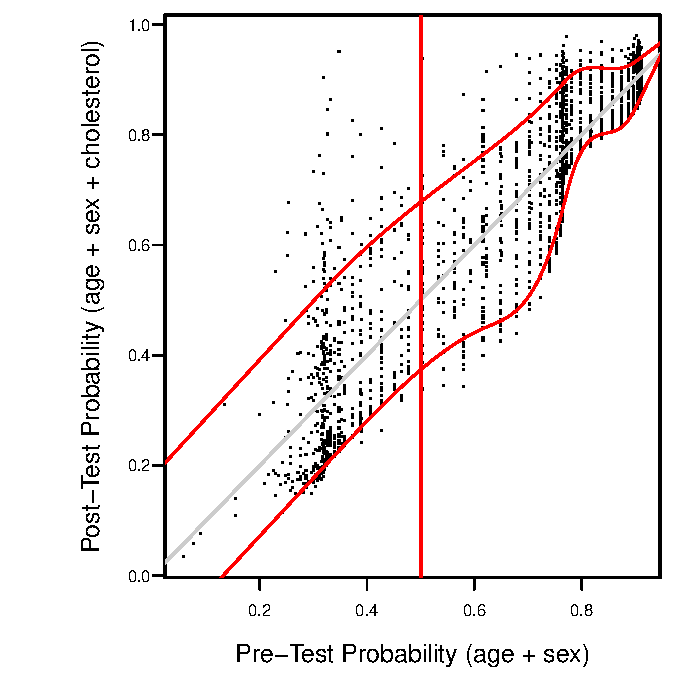
\includegraphics[width=\maxwidth]{dx-du-acath-1} }

\caption[Diagnostic Utility of Cholesterol for Diagnosing Significant CAD]{Diagnostic Utility of Cholesterol for Diagnosing Significant CAD.  Curves are 0.1 and 0.9 quantiles from quantile regression using restricted cubic splines}\label{fig:dx-du-acath}
\end{figure}
\end{Schunk}

\section{Summary}
{\smaller Diagnostic utility needs to be estimated using measures of
relevance to individual decision makers.  Improper accuracy scoring rules lead to suboptimal decisions.  Traditional risk modeling is a powerful tool in this setting.  Cohort studies are ideal but useful measures can be obtained
even with oversampling.  Avoid categorization of any continuous or ordinal variables.}
